
\documentclass{beamer}
\usetheme{Singapore}
\usecolortheme[dark,accent=blue]{solarized}
\setbeamertemplate{navigation symbols}{\insertframenumber}

\usepackage{hyperref, tikz}
\usetikzlibrary{arrows.meta, shapes.geometric}
\tikzset{>={To[length=3mm,width=3mm]}}

\title{Swinging, Fast and Slow}
\author{Scott Powers\inst{1} and Ron Yurko\inst{2}}
\date{Saberseminar 2024}
\institute{
  \inst{1} Department of Sport Management, Rice University \and
  \inst{2} Department of Statistics \& Data Science, Carnegie Mellon University
}
\begin{document}

\begin{frame}
    \maketitle
    \vfill\hfill
\includegraphics[width = 4cm]{../images/rice_logo_white.png}
\end{frame}

\begin{frame}{Question}
  How much do batters change their swings according to the count?\\
  ~\\
  And what are the consequences of these approaches?
\end{frame}

\begin{frame}{Conclusions (Preview)}
  \begin{enumerate}
    \item Estimating batter \alert{intention} is a helpful framework for reasoning about the sources of variation in swing metrics
    \item Batters can reduce their strikeout rate by modulating their swing length according to the count ...
    \item ... but it's not worth the power tradeoff for the average batter (from a linear weights perspective)
  \end{enumerate}
\end{frame}

\begin{frame}{Data}
  May 2024: MLB releases exciting new swing tracking metrics
  \begin{itemize}
    \item For every swing, we get:
    \begin{itemize}
      \item Swing length (distance traveled by bat head from ``start'')
      \item Bat speed (speed of bat ``sweet spot'')
    \end{itemize}
    \item Measured at point of contact (or point of nearest contact)
    \item Additional derived metrics:
    \begin{itemize}
      \item Squared-up rate (exit velocity $> 80\%$ of theoretical max)
      \item Fast-swing rate
      \item Blasts
      \item Swords
    \end{itemize}
    \item More in the future pipeline? (miss distance, contact depth, ...)
  \end{itemize}
  \begin{center}
    \alert{THANK YOU, MLBAM!}
  \end{center}
\end{frame}

\begin{frame}{When batters swing slower, do they make better contact?}
  \begin{center}
    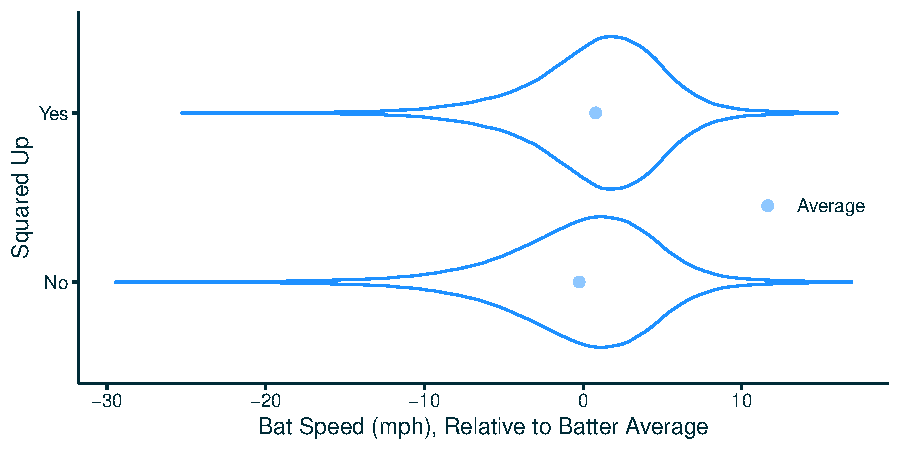
\includegraphics[width = \textwidth]{../../figures/beamer/counterintuitive.pdf}
  \end{center}
  \begin{itemize}
    \item Squared Up swings are faster on average, but ...
  \end{itemize}
\end{frame}

\begin{frame}{Caution \#1: Correlation does not imply causation}
  One possible causal model:
  \begin{center}
    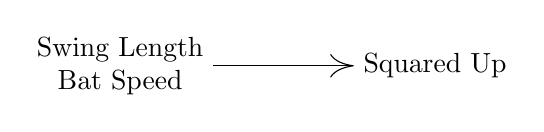
\begin{tikzpicture}[->, align = center]
      \node (swing_metrics) at (0, 0) {Swing Length \\ Bat Speed};
      \node (squared_up) at (4, 0) {Squared Up};
      \draw (swing_metrics) -- (squared_up);
    \end{tikzpicture}
  \end{center}
  Another (more plausible) causal model with confounders:
  \begin{center}
    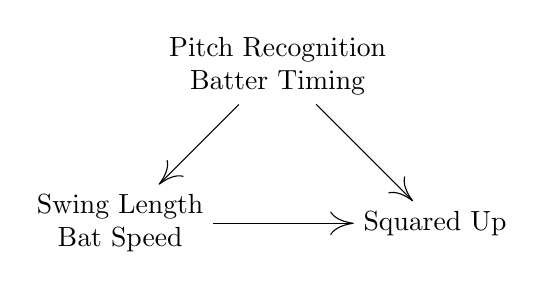
\begin{tikzpicture}[->, align = center]
      \node (confounders) at (2, 2) {Pitch Recognition \\ Batter Timing};
      \node (swing_metrics) at (0, 0) {Swing Length \\ Bat Speed};
      \node (squared_up) at (4, 0) {Squared Up};
      \draw (confounders) -- (swing_metrics);
      \draw (confounders) -- (squared_up);
      \draw (swing_metrics) -- (squared_up);
    \end{tikzpicture}
  \end{center}
\end{frame}

\begin{frame}{Caution \#2: How do we get our measurement?}
  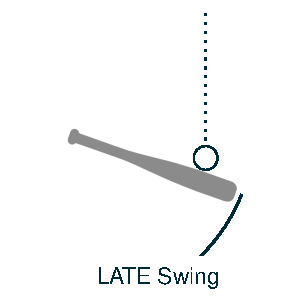
\includegraphics[width = 0.49\textwidth]{../../figures/beamer/swing_late.pdf}
  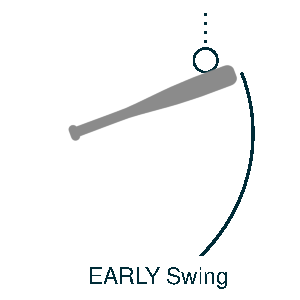
\includegraphics[width = 0.49\textwidth]{../../figures/beamer/swing_early.pdf}
  \begin{itemize}
    \item For \alert{identical} swings, timing determines point of measurement
    \item Swing length and bat speed are \alert{outcomes}, not purely process
  \end{itemize}
\end{frame}

\begin{frame}{Outline}
  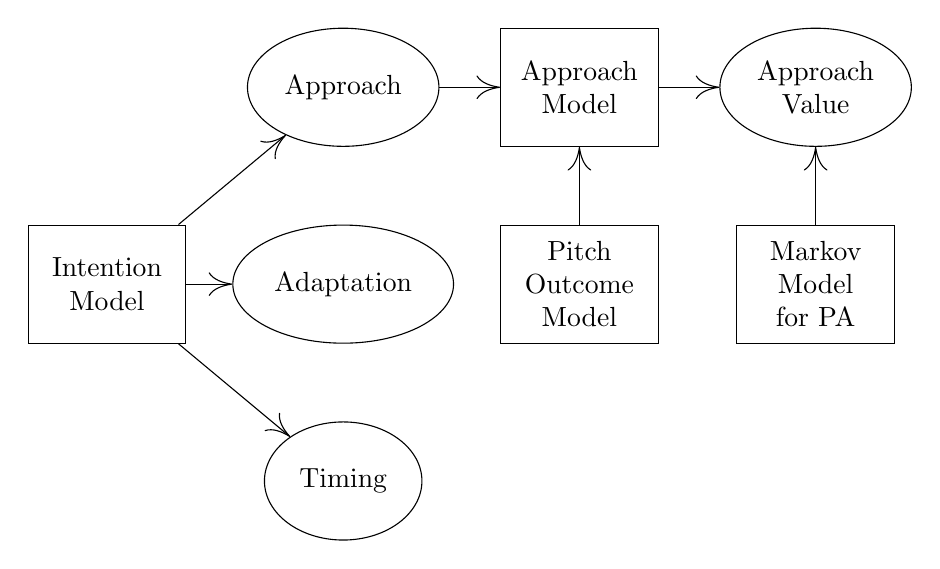
\begin{tikzpicture}[
    ->,
    align = center,
    minimum height = 1.5cm,
    minimum width = 2cm,
    every node/.style = {draw},
    model/.style = {rectangle},
    value/.style = {ellipse},
    alert/.style = {thick, draw = solarizedAccent}
  ]
    \node[model] (intention_model) at (0, 0) {Intention\\Model};
    \node[value] (approach) at (3, 2.5) {Approach};
    \node[value] (adaptation) at (3, 0) {Adaptation};
    \node[value] (timing) at (3, -2.5) {Timing};
    \node[model] (pitch_outcome_model) at (6, 0) {Pitch\\Outcome\\Model};
    \node[model] (approach_model) at (6, 2.5) {Approach\\Model};
    \node[model] (markov_model) at (9, 0) {Markov\\Model\\for PA};
    \node[value] (approach_value) at (9, 2.5) {Approach\\Value};
    \draw (intention_model) -- (approach);
    \draw (intention_model) -- (adaptation);
    \draw (intention_model) -- (timing);
    \draw (pitch_outcome_model) -- (approach_model);
    \draw (approach) -- (approach_model);
    \draw (markov_model) -- (approach_value);
    \draw (approach_model) -- (approach_value);
  \end{tikzpicture}
\end{frame}

\begin{frame}{Outline}
  \begin{tikzpicture}[
    ->,
    align = center,
    minimum height = 1.5cm,
    minimum width = 2cm,
    every node/.style = {draw},
    model/.style = {rectangle},
    value/.style = {ellipse},
    alert/.style = {thick, draw = solarizedAccent}
  ]
    \node[model, alert] (intention_model) at (0, 0) {\alert{Intention}\\\alert{Model}};
    \node[value] (approach) at (3, 2.5) {Approach};
    \node[value] (adaptation) at (3, 0) {Adaptation};
    \node[value] (timing) at (3, -2.5) {Timing};
    \node[model] (pitch_outcome_model) at (6, 0) {Pitch\\Outcome\\Model};
    \node[model] (approach_model) at (6, 2.5) {Approach\\Model};
    \node[model] (markov_model) at (9, 0) {Markov\\Model\\for PA};
    \node[value] (approach_value) at (9, 2.5) {Approach\\Value};
    \draw (intention_model) -- (approach);
    \draw (intention_model) -- (adaptation);
    \draw (intention_model) -- (timing);
    \draw (pitch_outcome_model) -- (approach_model);
    \draw (approach) -- (approach_model);
    \draw (markov_model) -- (approach_value);
    \draw (approach_model) -- (approach_value);
  \end{tikzpicture}
\end{frame}

\begin{frame}{Intention Model}
  Goal: Estimate swing metrics at intended point of contact
  \begin{enumerate}
    \item Filter on swings above 50 mph (avoid bunts, check-swings)
    \item Filter on swings that are squared-up (avoid bad timing)
    \item Fit mixed-effects linear models for swing length and bat speed
    \begin{itemize}
      \item Fixed and random effects for intercept, count, pitch location
    \end{itemize}
  \end{enumerate}
  \begin{align*}
    (\mbox{swing length})_i = \alpha &+ \gamma^A_{b_i}\\
        & \left.
          \begin{array}{l}
            +~\beta^B \cdot (\mbox{balls})_i\\
            +~(\beta^S + \gamma^S_{b_i}) \cdot (\mbox{strikes})_i
          \end{array}\color{solarizedAccent}
        \right\}\mbox{\alert{approach}}\\
        & \left.
          \begin{array}{l}
            +~(\beta^X + \gamma^X_{b_i}) \cdot (\mbox{pitch loc x})_i\\
            +~(\beta^Z + \gamma^Z_{b_i}) \cdot (\mbox{pitch loc z})_i
          \end{array}\color{solarizedAccent}
        \right\}\mbox{\alert{adaptation}}\\
        & \left.
          \begin{array}{l}
            +~\epsilon_i
          \end{array}
        \right.
  \end{align*}
\end{frame}

\begin{frame}{Approach: How do intended swings vary by count?}
  \centering
  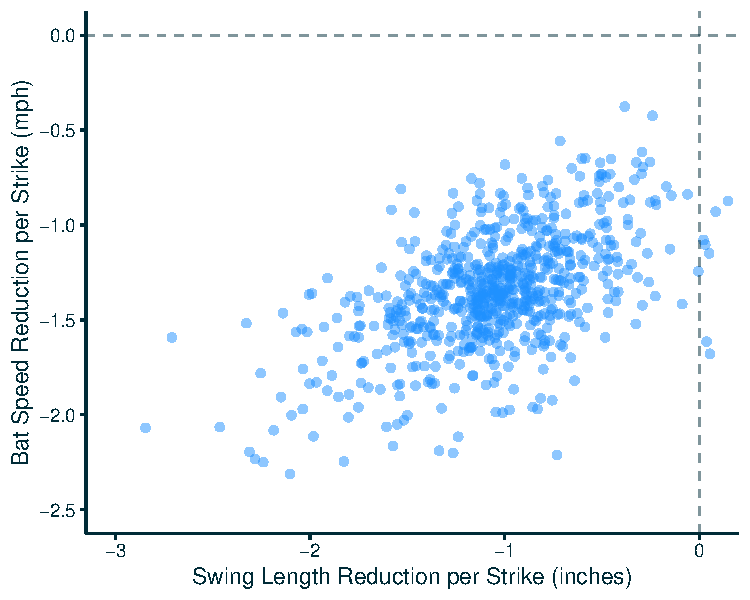
\includegraphics[height = 0.8\textheight]{../../figures/beamer/approach.pdf}
\end{frame}

\begin{frame}{Adaptation: How do intended swings vary by location?}
  \centering
  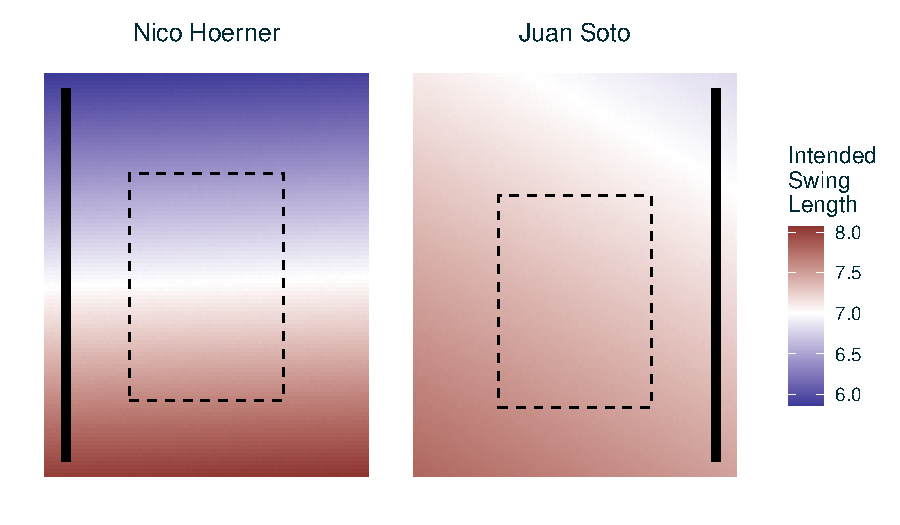
\includegraphics[width = \textwidth]{../../figures/beamer/adaptation.pdf}
  \begin{itemize}
    \item There's clearly a difference, but it's hard to say why
  \end{itemize}
\end{frame}

\begin{frame}{Timing: What swing variation remains unexplained?}
  \includegraphics[width = 0.49\textwidth]{../../figures/beamer/swing_metrics_intended.pdf}
  \includegraphics[width = 0.49\textwidth]{../../figures/beamer/swing_metrics_residual.pdf}
  \begin{itemize}
    \item Left: Predicted intention for all swings (not just squared up)
    \item Right: Residuals (relative to intention) for all swings
    \begin{itemize}
      \item Pattern matches bat speed through path of swing!
    \end{itemize}
  \end{itemize}
\end{frame}

\begin{frame}{Outline}
  \begin{tikzpicture}[
    ->,
    align = center,
    minimum height = 1.5cm,
    minimum width = 2cm,
    every node/.style = {draw},
    model/.style = {rectangle},
    value/.style = {ellipse},
    alert/.style = {thick, draw = solarizedAccent}
  ]
    \node[model] (intention_model) at (0, 0) {Intention\\Model};
    \node[value] (approach) at (3, 2.5) {Approach};
    \node[value] (adaptation) at (3, 0) {Adaptation};
    \node[value] (timing) at (3, -2.5) {Timing};
    \node[model] (pitch_outcome_model) at (6, 0) {Pitch\\Outcome\\Model};
    \node[model, alert] (approach_model) at (6, 2.5) {\alert{Approach}\\\alert{Model}};
    \node[model] (markov_model) at (9, 0) {Markov\\Model\\for PA};
    \node[value] (approach_value) at (9, 2.5) {Approach\\Value};
    \draw (intention_model) -- (approach);
    \draw (intention_model) -- (adaptation);
    \draw (intention_model) -- (timing);
    \draw (pitch_outcome_model) -- (approach_model);
    \draw (approach) -- (approach_model);
    \draw (markov_model) -- (approach_value);
    \draw (approach_model) -- (approach_value);
  \end{tikzpicture}
\end{frame}

\begin{frame}{Approach Model}
  \begin{enumerate}
    \item Start with pitch outcome model which estimates $\mathbb{P}$(swing), $\mathbb{P}$(contact $\mid$ swing), $\mathbb{P}$(fair $\mid$ contact), $\mathbb{E}$(xwOBA $\mid$ fair), etc.
    \begin{itemize}
      \item Gradient boosting w/ 2022-2024 MLB data
    \end{itemize}
    \item Refit contact, fair and xwOBA models on batter approach, with previous predictions as offset
  \end{enumerate}
  Example: $p_i$ is contact prob, $\hat p_i$ is pitch outcome model estimate
  \begin{align*}
    \log\left(\frac{p_i}{1 - p_i}\right) = \log\left(\frac{\hat p_i}{1 - \hat p_i}\right)
      &+ \beta^{SL} \cdot \hat\gamma^{SL}_{b_i} \cdot (\mbox{strikes})_i\\
      &+ \beta^{BS} \cdot \hat\gamma^{BS}_{b_i} \cdot (\mbox{strikes})_i
  \end{align*}
  \begin{itemize}
    \item This is instrumental variable regression from causal inference, using count as the instrument
  \end{itemize}
\end{frame}

\begin{frame}{The Effect of Approach}{``Effect'' is approach-aware vs. approach-agnostic prediction w/ 2 strikes}
  \centering
  \includegraphics[width = 0.49\textwidth]{../../figures/beamer/swing_length_contact.pdf}
  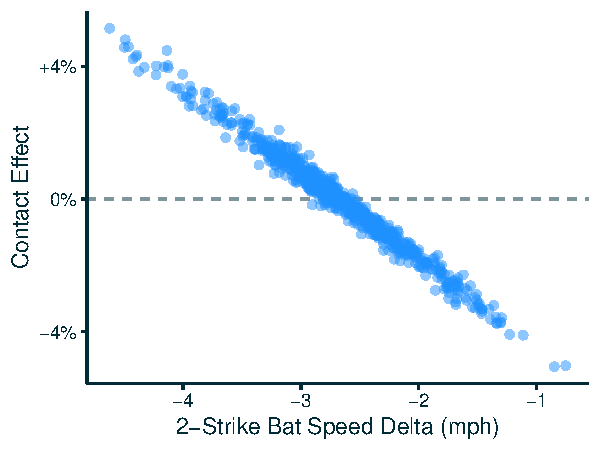
\includegraphics[width = 0.49\textwidth]{../../figures/beamer/bat_speed_contact.pdf}\\
  \includegraphics[width = 0.49\textwidth]{../../figures/beamer/swing_length_power.pdf}
  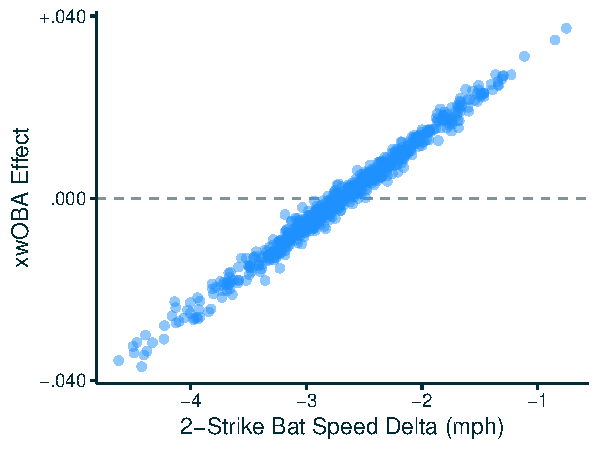
\includegraphics[width = 0.49\textwidth]{../../figures/beamer/bat_speed_power.pdf}
\end{frame}

\begin{frame}{Outline}
  \begin{tikzpicture}[
    ->,
    align = center,
    minimum height = 1.5cm,
    minimum width = 2cm,
    every node/.style = {draw},
    model/.style = {rectangle},
    value/.style = {ellipse},
    alert/.style = {thick, draw = solarizedAccent}
  ]
    \node[model] (intention_model) at (0, 0) {Intention\\Model};
    \node[value] (approach) at (3, 2.5) {Approach};
    \node[value] (adaptation) at (3, 0) {Adaptation};
    \node[value] (timing) at (3, -2.5) {Timing};
    \node[model] (pitch_outcome_model) at (6, 0) {Pitch\\Outcome\\Model};
    \node[model] (approach_model) at (6, 2.5) {Approach\\Model};
    \node[model, alert] (markov_model) at (9, 0) {\alert{Markov}\\\alert{Model}\\\alert{for PA}};
    \node[value] (approach_value) at (9, 2.5) {Approach\\Value};
    \draw (intention_model) -- (approach);
    \draw (intention_model) -- (adaptation);
    \draw (intention_model) -- (timing);
    \draw (pitch_outcome_model) -- (approach_model);
    \draw (approach) -- (approach_model);
    \draw (markov_model) -- (approach_value);
    \draw (approach_model) -- (approach_value);
  \end{tikzpicture}
\end{frame}

\begin{frame}{Is it good to modulate your swing by count?}
  \centering
  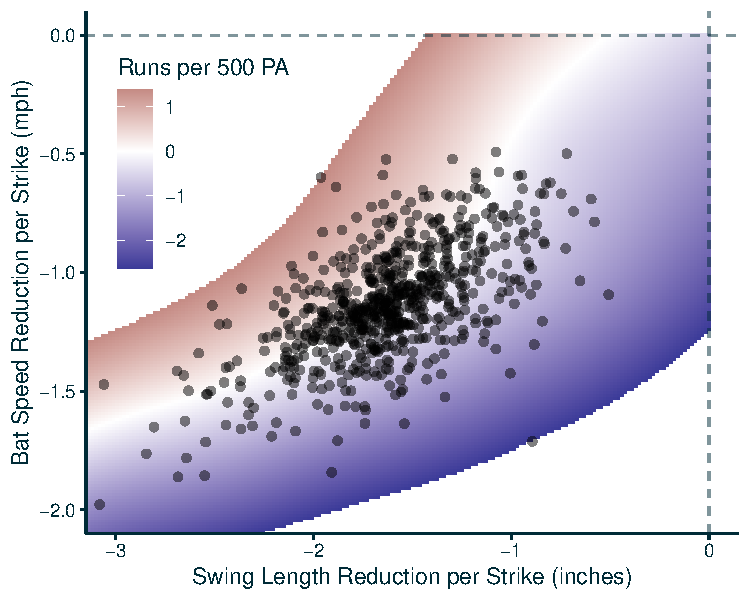
\includegraphics[height = 0.9\textheight]{../../figures/beamer/approach_run_value.pdf}
\end{frame}

\begin{frame}{Is it good to modulate your swing by count?}
  \centering
  \includegraphics[height = 0.9\textheight]{../../figures/beamer/approach_run_value_labelled.pdf}
\end{frame}

\begin{frame}{Conclusions}
  \begin{enumerate}
    \item Estimating batter \alert{intention} is a helpful framework for reasoning about the sources of variation in swing metrics
    \item Batters can reduce their strikeout rate by modulating their swing length according to the count ...
    \item ... but it's not worth the power tradeoff for the average batter (from a linear weights perspective)
  \end{enumerate}
\end{frame}

\begin{frame}{Thank You!}
  Acknowledgements: Nick Wan, Noah Woodward\\
  ~\\
  All code for this project (and these slides) available at:\\
  \alert{\url{github.com/saberpowers/swinging-fast-and-slow}}\\
  ~\\
  You can learn more about each of our research at:\\
  \alert{
    \url{saberpowers.github.io}\\
    \url{stat.cmu.edu/~ryurko}
  }
\end{frame}

\end{document}
